% Chapter 3

\chapter{Geles polim\'ericos} % Main chapter title

\label{Chapter-geles} % For referencing the chapter elsewhere, use \ref{Chapter1} 

%----------------------------------------------------------------------------------------

% Define some commands to keep the formatting separated from the content 
\newcommand{\keyword}[1]{\textbf{#1}}
\newcommand{\tabhead}[1]{\textbf{#1}}
\newcommand{\code}[1]{\texttt{#1}}
\newcommand{\file}[1]{\texttt{\bfseries#1}}
\newcommand{\option}[1]{\texttt{\itshape#1}}

%----------------------------------------------------------------------------------------




\section{Introducci\'on/Motivaci\'on}


Como hemos mencionado en la introducci\'on de este tesis los micro-nanogeles polim\'ericos son sistemas polim\'ericos que presentan una estructura tridimensional en forma de red. Estos geles se forman mediante la reticulaci\'on de pol\'imeros (o copol\'imeros), lo que da lugar a una matriz de pol\'imero tridimensional que puede retener grandes cantidades de agua o solventes.
Estos sitemas  representan una plataforma vers\'atil y prometedora para diversas aplicaciones biom\'edicas. Su capacidad para retener agua y solventes, su tama\~no nanom\'etrico y su capacidad de funcionalizaci\'on los convierten en sistemas atractivos para la entrega de f\'armacos
Este sistema de delivery requiero el entendimiento de la fisicoqu\'imica que engloba todo el proceso.
Desde el proceso de encapsaludo hasta posibles mecanismos de liberaci\'on en los lugares deseseados.
Con esto nos referimos a entender que tipo de interacciones existen y predominan y hacen que el proceso se lleve a cabo.

En este cap\'itulo mostramos el desarrollo de una teor\'ia de equilibrio de dos fases y realizamos una investigaci\'on sistem\'atica del comportamiento termodin\'amico de microgeles compuestos de copol\'imeros aleatorios de NIPAm y un comon\'omero \'acido (MAA).
Este modelo describe la qu\'imica f\'isica detr\'as de todos los fen\'omenos de hinchamiento del microgel impulsado por el pH, la dependencia no monot\'onica del tama\~no de part\'icula de la concentraci\'on de sal y el colapso de la red al aumentar la temperatura por encima del VPTT.
Las predicciones que mostramos brindan una imagen clara de los efectos de la composici\'on de la soluci\'on (pH, concentración de sal) y la qu\'imica del pol\'imero (contenido de MAA, grado de entrecruzamiento) en el VPT.
Tambi\'en investigamos las mejores condiciones para la encapsulaci\'on de doxorrubicina y daunorrubicina dentro de estos microgeles.
Los c\'alculos  ac\'a mostrados son espec\'ificos para el \'acido metacr\'ilico con $pKa = 4,65$, pero el comportamiento fisicoqu\'imico informado puede describir cualitativamente una variedad de microgeles basados en NIPAm que se han modificado con otros mon\'omeros \'acidos que tienen diferente pka y diferente solubilidad a pH bajo.

El nivel de teor\'ia usado en este cap\'itulo corresponde a un sitema de dos fases, del tipo Donnan \cite{overbeek1956donnan}, en el cual la fase polim\'erica es considera homogenea. La fase soluci\'on con la que se encuentra en contacto contiene los iones y adsorbatos lso cuales pueden permear en la fase polim\'erica. En cambio nuestro gel no puede pasar a la fase soluci\'on. 
El sistema termodinamicamente hablando corresponde a un sistema semi-gran canonico que incluye todas las los terminos energeticos necesarios para una descripci\'on detallada del mismo. 
En las siguientes secciones se har\'a rese\~na sobre las ecuaciones que describen la fisicoqu\'imica del sistema. La descripci\'on se har\'a para cada una de las fases. En una tercera parte se mostrará como se ve modificada el potencial termodin\'amico del sistema cuando se consideran adsorbatos.  Los adsorbatos elegidos corresponden a dos drogas Doxorubucina y Daunorubicina. La elecci\'on de estas drogas debido a su alto uso en terapias anticancerigenas. Las mismas cuentan con estudios experimentales en microgeles de poli(NIPAm-co-MAA) para la encapsulaci\'on/liberaci\'on de estos f\'armacos. \addcite[drogas]
Se har\'a enfasis en la optimización para su encapsulado en estos geles polimericos.  

\subsection{Teor\'ia: Fase Microgel}\label{sec:gel:theory}
%%%%%%%%%%%%%%%%%%%%%%%%%%%%%%%%%%%%%%%%%%%%%%%%%%%%%%%%%%%%%%%%%%%%%


Consideremos un modelo de dos fases: un microgel de poli(NIPAm-\emph{co}-MAA) (P(NIPAm-MAA)) (la fase $1$, denotada por $MG$) en contacto con una soluci\'on acuosa ( fase $2$, denotada por $s$).
Externamente, podemos controlar la temperatura $T$, el pH y la concentraci\'on de sal de esta soluci\'on, lo que da como resultado que el microgel tenga un radio $R$ y un volumen $V=\frac{4}{3}\pi R^3$.
El potencial termodin\'amico cuyo m\'inimo produce las condiciones de equilibrio dentro de la fase de microgel es un  potencial semi gran can\'onico, $\Omega_{MG}$.
%
\begin{align}
    \begin{aligned}
       \Omega_{MG}=& -TS_{mez} + F_{qca,MAA} +  F_{ela}\\
       & + U_{elec}+  U_{ste} + U_{VdW} -{\sum_{\gamma}
        {\mu_\gamma N_\gamma}}
    \end{aligned}
    \label{eq:gel:free-energy-implicit}
\end{align}
%

\noindent En donde $S_{mez}$ es la entropí\'ia de traslaci\'on (mezcla) de las especies libres en la fase de microgel: mol\'eculas de agua ($w$), hidronio ($H_3O^+$) e iones de hidr\'oxido ($OH^-$ ), y cationes de sal ($+$) y aniones ($-$).
Hemos considerado una sal monovalente, $KCl$,  completamente disociada en iones de potasio y cloruro.

\begin{align}
-\frac{S_{mez}}{k_B}	= \sum_{\gamma} \rho_\gamma\left(\ln\left(\rho_\gamma v_w\right) -1 + \beta\mu^0_\gamma\right) 
\end{align}

\noindent en donde  $\beta=\frac{1}{k_BT}$ , $T$ es la temperatura del sisteman y  $k_B$ es la constante de Boltzmann.
La densidad num\'erica de la especie $\gamma$ es $\rho_\gamma$ y $\mu^0_\gamma$ es su potencial qu\'imico est\'andar,  $v_w$ es el volumen de una mol\'ecula de agua.

$F_{qca,MAA}$ es la energ\'ia química libre que describe la protonaci\'on de equilibrio de las unidades de MAA.


\begin{align}
	\beta F_{qca, MAA} =  \frac{\phi_{MAA}}{v_{MAA}} \left[f(\ln f+ \beta\mu^0_{MAA^-}) +(1-f)(\ln (1-f)+\beta\mu^0_{MAAH})\right]
\end{align}


\noindent donde $\phi_{MAA}$ es la fracci\'on de volumen que ocupan estos segmentos, $v_{MAA}$ es el volumen de este segmento, y $f$ es el grado de disociaci\'on del mismo. 
La fracci\'on de volumen de los segmentos MAA cargados es $f\phi_{MAA}$, y la de las unidades protonadas (o sin carga) es $(1-f)\phi_{MAA}$.
Los potenciales qu\'imicos est\'andar son $\mu^0_{MAA^-}$ y $\mu^0_{MAAH}$ para las especies desprotonadas(cargadas) y protonadas, respectivamente.
Utilizamos el t\'ermino segmento para identificar las unidades qu\'imicas que componen las cadenas polim\'ericas (MAA y NIPAm).


$F_{ela}$ es la energ\'ia libre el\'astica que explica la libertad conformacional de la red polim\'erica.

\begin{align}
	\beta F_{ela} = \dfrac{3}{2}\dfrac{N_{seg}}{n_{ch} V}\left[\left(\dfrac{R}{R_0}\right)^2 - \ln\dfrac{R}{R_0} -1\right]
\end{align}

Esta expresi\'on se describe en \cite{moncho-jorda2016a} y proviene del modelo de elasticidad del caucho,
donde $N_{seg}$ es el n\'umero total de segmentos en la red de pol\'imero y $n_{ch}$ es el n\'umero de segmentos por cadena de pol\'imero o \emph{longitud de cadena}.
La constante de elasticidad en esta energ\'ia es proporcional al cociente $\dfrac{N_{seg}}{n_{ch}}$, que representa el n\'umero (total) de cadenas de pol\'imero en el microgel.
El radio del microgel seco es $R_0$, lo que satisface con la expresi\'on:

%
%
\begin{align}
	\begin{aligned} 
		\dfrac{4}{3}\pi R_0^3=V_0&=N_{seg}\Big( x_{MAA} v_{MAA}\\
		&\qquad+x_{NIPAm} v_{NIPAm}\Big)
	\end{aligned}
\end{align}


\noindent donde $V_0$ es el volumen de la part\'icula seca; $x_{MAA}$ y $x_{NIPAm}$ son la fracci\'on de los segmentos MAA y NIPAm, respectivamente.
Entonces, el n\'umero total de segmentos MAA es $x_{MAA}N_{seg}$ y el de unidades NIPAm es $x_{NIPAm}N_{seg}$, cada uno con un volumen $v_{NIPAm}$.
Los microgeles que consideramos aqu\'i satisfacen $x_{NIPAm}=1-x_{MAA}$.



$U_{elec}$ y $U_{ste}$ representan respectivamente las interacciones electrost\'aticas y las repulsiones est\'ericas.

\begin{align}
	  \beta U_{elec} =\left(\sum_{\gamma } {\rho_\gamma q_\gamma + f\dfrac{\phi_{MAA}}{v_{MAA}}q_{MAA}}\right)\beta\psi_{MG}
\end{align}

\noindent donde $q_\gamma$ y $q_{MAA}$ son la carga el\'ectrica de las moléculas $\gamma$ y los segmentos MAA, respectivamente.
El potencial electrost\'atico dentro de la fase de microgel es $\psi_{MG}$. Fuera de esta fase el potencial es nulo $\psi_s = 0$

En donde se impone una restriccio\'on de electroneutralidad del microgel, que puede expresarse como:
%
%
\begin{align}
	\begin{aligned}
		\sum_{\gamma  } \rho_\gamma q_\gamma + f\frac{\phi_{MAA}}{v_{MAA}}q_{MAA}=0
	\end{aligned}
	\label{eq:gel:charge-neutrality}
\end{align}

Las interacciones stericas se incorporan como una segunda restricci\'on al sistema, la cual consiste en que  el volumen del microgel est\'a completamente ocupado por los segmentos de la red y las especies quí\'icas libres.

%
\begin{align}
	\begin{aligned}
		\sum_{\gamma } \rho_\gamma v_\gamma  + \phi_{MAA} + \phi_{NIPAm} = 1
	\end{aligned}
	\label{eq:gel:packing}
\end{align}



\noindent donde $v_\gamma$  es el volumen molecular de la especie $\gamma$, y la fracci\'on de volumen de cada componente de la red son: 
%
%
\begin{align}
	\phi_{MAA}&=N_{seg}\dfrac{x_{MAA}v_{MAA}}{\frac{4}{3}\pi R^3}\\
	\phi_{NIPAm}&=N_{seg}\dfrac{x_{NIPAm}v_{NIPAm}}{\frac{4}{3}\pi R^3}
\end{align}



$U_{VdW}$ es la contribuci\'on que describe las interacciones efectivas pol\'imero-disolvente; para este trabajo hemos realizado la siguiente aproximaci\'on: 
\begin{align}
	U_{VdW} = U_{NIPAm-w} + U_{MAA-w}
\end{align}
\noindent en donde $U_{NIPAm-w}$ incorpora la transici\'on hidrofílica-hidrof\'obica de NIPAm al aumentar la temperatura por encima de su temperatura de transici\'on cr\'itica. 
Del mismo modo $U_{MAA-w}$ hace cuenta de la interacci\'on entre los segmentos de MAA y agua.
Los resultados presentes en este cap\'itulo consideran a los segmentos de $MAA$ completamente hidrofilicos y por tanto $U_{MAA-w} = 0$

\begin{align}
	\beta U_{VdW} = U_{NIPAm-w} = \chi (T, \phi_{NIPAm})\rho_w \phi_{NIPAm}
\end{align}


Este  t\'ermino explica la respuesta de PNIPAm a los cambios de temperatura a trav\'es de un par\'ametro de interacci\'on pol\'imero solvente, $\chi$, que depende de la temperatura y la fracci\'on de volumen de NIPAm, $\phi_{NIPAm}$.
Seg\'un  \citet{afroze2000}, este par\'ametro de Flory-Huggins se puede expresar como:
%
%


\begin{align}
	\begin{aligned}
		\chi (T, \phi_{NIPAm}) &=g_0(T) +g_1(T)\phi_{NIPAm} \\
		&~+ g_2(T)\phi_{NIPAm}^2
	\end{aligned}
\end{align}

\noindent con
%
%
\begin{align}
	\begin{aligned} 
		g_k(T)=g_{k0} + \frac{g_{k1}}{T} + g_{k2}T
	\end{aligned}
\end{align}


\noindent para  $k=0,1,2$, los coeficinetes son: $g_{00}= -12.947$, $g_{02}=0.044959\,$K$^{-1}$, $g_{10}= 17.920$, $g_{12}= -0.056944$\,K$^{-1}$, $g_{20}= 14.814$, $g_{22}= -0.051419$\,K$^{-1}$  y $g_{k1}\equiv 0$ \cite{afroze2000}




Finalmente, la suma sobre  $\gamma$ expresa el equilibrio qu\'imico con la fase de soluci\'on, donde $\mu_\gamma$ y $N_\gamma$ son el potencial qu\'imico y el n\'umero de mol\'eculas de la especie $\gamma$, respectivamente.
Aqu\'i, el subíndice $\gamma$ identifica  las especies qu\'imicas libres, $\gamma \in \left\{ w, H_3O^+, OH^-, +,- \right\}$.
Hay que tener en cuenta que $\Omega_{MG}$ es un potencial semi-gran can\'onico porque la fase de microgel puede intercambiar cada una de estas mol\'eculas con la fase de soluci\'on, mientras que la red de pol\'imero está confinada dentro de la primera.


\begin{align}
	\sum_\gamma N_\gamma \mu_\gamma = \sum_{\gamma }{\rho_\gamma\beta\mu_\gamma}
	+ \beta\mu_{H^+}(1-f)\dfrac{\phi_{MAA}}{v_{MAA}}
\end{align}

Esta contribuci\'on muestra el equilibrio qu\'imico entre el microgel y la fase de soluci\'on, donde el segundo t\'ermino representa a los protones asociados a unidades de MAA;
a saber, $\mu_{H^+}\equiv\mu_{H_3O^+}$ se conjuga con el n\'umero total de protones,
$N_{H_3O^+}+N_{MAAH}=V\left(\rho_{H_3O^+}+(1-f)\dfrac{\phi_{MAA}}{v_{MAA}}\right)$.


La forma expl\'icita del potencial termodin\'amico es:




%
\begin{align}
\begin{aligned}
\beta&\frac{\Omega_{MG}(R)}{V}=\\& ~ \sum_{\gamma} \rho_\gamma\left(\ln\left(\rho_\gamma v_w\right) -1 + \beta\mu^0_\gamma\right) \\
& + \frac{\phi_{MAA}}{v_{MAA}} \left[f(\ln f+ \beta\mu^0_{MAA^-})\right.\\
&\qquad\left.+(1-f)(\ln (1-f)+\beta\mu^0_{MAAH})\right] \\
%
& + \dfrac{3}{2}\dfrac{N_{seg}}{n_{ch} V}\left[\left(\dfrac{R}{R_0}\right)^2 - \ln\dfrac{R}{R_0} -1\right] \\
%
& +  \left(\sum_{\gamma } {\rho_\gamma q_\gamma + f\dfrac{\phi_{MAA}}{v_{MAA}}q_{MAA}}\right)\beta\psi_{MG}\\
%
& +\beta\pi_{MG} \left[ \sum_{\gamma } \rho_\gamma v_\gamma  + \phi_{MAA} + \phi_{NIPAm} -1 \right] \\
%
& + \chi (T, \phi_{NIPAm})\rho_w \phi_{NIPAm} \\
%
& -\sum_{\gamma }{\rho_\gamma\beta\mu_\gamma}
 -\beta\mu_{H^+}(1-f)\dfrac{\phi_{MAA}}{v_{MAA}}\\
%
%
\end{aligned}
\label{eq:gel:free-energy}
\end{align}




\noindent En donde $\pi_{MG}$ es la presi\'on osm\'otica de la fase de microgel, introducido como un multiplicador de Lagrange para imponer la restricci\'on de incompresibilidad, ec. \ref{eq:gel:packing}.


Nuestro potencial termodin\'amico esta explicitamente en funci\'on de las densidades de todas las especies, el grado de carga del MAA y el radio del microgel, $\Omega_{MG}(R)\equiv\Omega_{MG}(\{\rho_\gamma\},f,R)$.
Para obtener las expresiones de $\{\rho_\gamma\}$ y $f$ de tal forma que sean consistentes con el equilibrio termodin\'amico, minimizamos $\Omega_{MG}$ respecto a estas cantidades, y  sujeto a las restricciones ec. \ref{eq:gel:packing} y ec. \ref{eq:gel:charge-neutrality}; dicho procedimiento conduce a: 
%
%
\begin{align}
\rho_\gamma v_w &= a_\gamma \exp(-\beta\pi_{MG}v_\gamma -\beta\psi_{MG}q_{\gamma})\\
\frac{f}{1-f}&= \frac{K^0_{MAA}}{a_{H^+}}\exp(-\beta\psi_{MG}q_{MAA})\label{eq:gel:fcharge}
\end{align}

\noindent donde $a_\gamma = e^{\beta\mu_\gamma-\beta\mu_\gamma^0}$ es la actividad de la especie $\gamma$. 
La constante de equilibrio termodin\'amico que describe la protonaci\'on/desprotonaci\'on MAA es
%
%
\begin{align}
K^0_{MAA}= e^{\beta\mu^0_{MAAH}-\beta\mu^0_{MAA}-\beta\mu^0_{H^+}}
\end{align}

\noindent Esta cantidad es posible calcularla directamente a partir del pKa del \'acido.


Si se considera  un valor de  $R$, las \'unicas inc\'ognitas restantes para determinar $\Omega_{MG}(R)$ son la presi\'on osm\'otica, $\pi_{MG}$ y el potencial electrost\'atico, $\psi_{MG}$.
Estas dos cantidades se pueden calcular resolviendo num\'ericamente la incompresibilidad y la electroneutralidad de la fase de microgel, ec. \ref{eq:gel:packing} y ec. \ref{eq:gel:charge-neutrality}, respectivamente.
Para resolver estas ecuaciones utilizamos un m\'etodo h\'ibrido de Powell sin jacobiano y un c\'odigo FORTRAN desarrollado internamente.
En resumen, es posible calcular la variaci\'on de energ\'ia potencial respecto del radio del microgel $R$, y con ello calcular el valor del radio \'optimo del gel para unas condiciones dadas( pH, temperatura, concentraci\'on de sal). Esto se ilustra en la secci\'on \ref{sec:gel:minimi}.

Todas las dem\'as cantidades involucradas en el c\'alculo de $\Omega_{MG}(R)$ son valores de  entradas, incluidas las propiedades de las diferentes especies qu\'imicas consideradas, que se resumen en la tabla \ref{table:gel:molecules}.
Usamos $pK_w=14$ para describir el equilibrio de disociaci\'on del agua.
Las actividades de todas las especies qu\'imicas libres se pueden calcular a partir de la concentraci\'on de estas mol\'eculas en la fase de soluci\'on, como se analiza a continuaci\'on.


\begin{table}
	\centering
%\small
%\begin{tabular}{lcS[table-format=-1]S[table-format=0.3]}
\begin{tabular}{|lccc|}
    \hline
    {Species} & {$pKa$} & {$q$ ($e$)} & {$v$ ($\text{nm}^3$)} \\
      \hline
$H_2O\,(w)$ & ~ & ~ & 0.03\\
$H_3O^+$ & ~ & +1 & 0.03\\
$OH^-$ & ~ & -1 & 0.03\\
$K^+\,(+)$ & ~ & +1 & 0.04\\ 
$Cl^-\,(-)$ & ~ & -1 & 0.047\\
$MAA$ & 4.65 & -1$^\ast$ & 0.09\\
$NIPAm$ & ~ & ~ & 0.12\\
    \hline
  \end{tabular}
 \caption{Propiedades moleculares de las diferentes especies qu\'imicas consideradas.
 	\footnotesize ($^\ast$Para las especies desprotonadas).}
\label{table:gel:molecules} 
\end{table}


%%%%%%%%%%%%%%%%%%%%%%%%%%%%%%%%%%%%%%%%%%%%%%%%%%%%%%%%%%%%%%%%%%%%%
\subsection{Fase soluci\'on}\label{sec:gel:fase-solucion}
%%%%%%%%%%%%%%%%%%%%%%%%%%%%%%%%%%%%%%%%%%%%%%%%%%%%%%%%%%%%%%%%%%%%%

En la soluci\'on, el potencial termodin\'amico es:
%
%
\begin{align}
\begin{aligned}
\beta&\frac{\Omega_s}{V}=\\& \sum_{\gamma   } {\rho^s_\gamma\left(\ln(\rho_\gamma^sv_w) -1 + \beta\mu_\gamma^0 - \beta\mu_\gamma\right)} \\
& +\beta\pi_{s} \left[ \sum_{\gamma } \rho_\gamma v_\gamma + \rho_a \sum_\lambda n_\lambda v_\lambda -1 \right] \\
\end{aligned}
\label{eq:gel:bulk}
\end{align}

\noindent el subindice  $s$  indica las densidades en la fase soluci\'on.
Al escribir la ec. \ref{eq:gel:bulk}, hemos considerado un volumen de referencia igual al del microgel, $V$, y se ha considerado, como se mencion\'o con anterioridad, cero el potencial electrost\'atico en la fase de soluci\'on.
Adem\'as en la ultima l\'inea de la ecuaci\'on \ref{eq:gel:bulk} se ha incorporado la restricci\'on para la incompresibilidad del sistema, con $pi_s$ como la presi\'on osm\'otica en la fase soluci\'on.

Una vez que se establece la composición de la soluci\'on (pH y concentraci\'on de sal), conocemos las densidades de todas las especies qu\'imicas en esta fase, que deben satisfacer tanto las restricciones de incompresibilidad como de neutralidad de carga:
%
%
\begin{align}
\sum_{\gamma  } \rho_\gamma^s v_\gamma  &=1\label{eq:gel:bulk-packing}\\
\sum_{\gamma  } \rho_\gamma^s q_\gamma  &=0
\end{align}

\noindent con
%
%
\begin{align}
\rho_\gamma^s v_w= a_\gamma \exp(-\beta\pi_s v_\gamma)
\label{eq:gel:bulk-electroneutrality}
\end{align}



\noindent para $\gamma \in \left\{ w, H_3O^+, OH^-, +,- \right\}$, donde $\pi_s$ es la presi\'on osm\'otica de la fase de soluci\'on introducida como un multiplicador de Lagrange por la ecuaci\'on \ref{eq:gel:bulk-packing}.
Al conocer $\pi_s$, podemos determinar las actividades de todas las especies qu\'imicas libres, y con las mismas resolver el sistema de la fase microgel.
Los resultados de la minimizaci\'on de la energ\'ia con un dado valor de R es presentada en la siguiente secci\'on.

\subsection{Minimizaci\'on gr\'afica}\label{sec:gel:minimi}
%%%%%%%%%%%%%%%%%%%%%%%%%%%%%%%%%%%%%%%%%%%%%%%%%%%%%%%%%%%%%%%%%%%%%

\begin{figure*}[!htb]
\centering
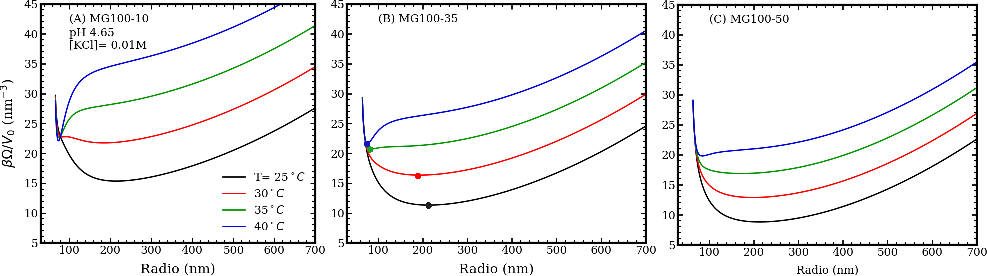
\includegraphics[width=1.\linewidth]{Figures/graph-gel/graph-min.pdf}
\caption{Potencial termodin\'amico en funci\'on del radio del microgel a diferentes temperaturas, $pH~4.65$ y $cs=10^{-2}M$.
	Cada panel corresponde a un microgel MG100 diferente (longitud de cadena, $n_{ch}=100$) con $10\%$ (A), $35\%$ (B) y $50\%$ (C) MAA.
	Las curvas presentan el potencial termodin\'amico en exceso de la contribuci\'on de la soluci\'on, $\Omega=\Omega_{MG}-\Omega_s$, en algunas unidades convenientes, donde $V_0=\frac{4}{3}\pi R_0^3$ es el volumen de la part\'icula polim\'erica seca.
	En el panel B, los puntos  marcan el radio \'optimo para cada temperatura, que es el m\'inimo local/global de la curva correspondiente (ver tabla \ref{table:gel:optimal-R}).}
\label{fig:gel:graph-min}
\end{figure*}

Como mencionamos en la secci\'on \ref{sec:gel:theory} es posible determinar completamente la energ\'ia libre de la fase de microgel para cualquier $R$ dado.
Las variables independientes en este c\'alculo son la temperatura, el pH y la concentraci\'on de sal de la soluci\'on en contacto con la fase microgel.
El n\'umero de segmentos en la red de pol\'imero $N_{seg}$, la longitud de la cadena $n_{ch}$ y la fracci\'on de segmentos MAA, $x_{MAA}$, caracterizan completamente a nuestro microgel, es decir son variables de entrada pre-establecidas.


Consideramos microgeles con $N_{seg}=10^7$ segmentos y $n_{ch}=50$, $100$ y $200$, que tienen $x_{MAA}=0,1$, $0,35$ o $0,5$.
En esta primera instancia evaluamos el efecto de aumentar o reducir la cantidad de mon\'omero \'acido con respecto a los microgeles de poli(NIPAm-\emph{co}-MAA) que tienen $35\%$ MAA.

Estos microgeles est\'an etiquetados como MG$n_{ch}$-$p_{MAA}$, donde $p_{MAA}$ es el porcentaje de MAA.
Por ejemplo, MG100-10 corresponde a un  microgel con $n_{ch}=100$ y $x_{MAA}=0,1$.


Para determinar el tama\~no del microgel para un conjunto dado de condiciones, recurrimos a una minimizaci\'on gr\'afica del mismo.
Para cada conjunto de condiciones (pH, sal y $T$), obtenemos la energ\'ia $\Omega(R)=\Omega_{MG}(R)-\Omega_{s}(R)$. En esta expresi\'on obtenemos el potencial termodin\'amico en exceso de la contribuci\'on energ\'etica de la soluci\'on.
Con ella podemos encontrar el $R_{opt }$, siedo este el radio \'optimo, tal que la curva tenga un m\'inimo local (y global).
Como ejemplo, este procedimiento se ilustra en la figura \ref{fig:gel:graph-min} para microgeles MG100.
Los resultados obtenidos de la minimizaci\'on de las curvas figura \ref{fig:gel:graph-min} se resumen en la tabla \ref{table:gel:optimal-R}.

\begin{table}[!htb]
\centering
\small
  \begin{tabular}{|lccccc|}
   \hline %\multirow{2}{*}{MG100} & 
    %  \multicolumn{4}{c}{Opt. Radius (nm)(MG100)} \\
    	&&   Radio \'optimo (nm)(MG100) & && \\
    	\hline
      & {25 $^\circ C$} & {30 $^\circ C$} & {35 $^\circ C$} & {40 $^\circ C$} & {Gel seco, $R_0$} \\
      \hline
    10\% MAA & 215 &  184 &  75  &  74 & 65\\
    35\% MAA &  213 &  193 &  84 & 76 & 64\\
    50\% MAA &  213 & 199 &  172 & 85 & 63\\
    \hline
  \end{tabular}
 \caption{Minimizaci\'on de las curvas de la  figura \ref{fig:gel:graph-min}.
 	Esta tabla resume los radios \'optimos de tres microgeles MG100 a diferentes temperaturas, $pH\,4.65$ y $[KCl]=10^{-2}M$.}
\label{table:gel:optimal-R} 
\end{table}


\subsection{Adsorci\'on de drogas}\label{sec:gel:adsorcion}
%%%%%%%%%%%%%%%%%%%%%%%%%%%%%%%%%%%%%%%%%%%%%%%%%%%%%%%%%%%%%%%%%%%%%

Nuestro objetivo es poder utilizar estos microgeles como dispositivos inteligentes, entre los que se destaca su uso como trasnportadores de mecidamentos. Para ello es necesario analizar su factibiliad de su adsorci\'on de algunas drogas terapeuticas. En el presente cap\'itulo realizamos el an\'alisis usando como droga modelo a la Doxorubicina y un derivado de ella: Daunorubicina. Ambas drogas muy fuertemente empleadas en tratamientos anticancerigenos. 

Para describir la adsorci\'on de un analito a la fase de microgel,
al potencial termodin\'amico de la ec. \ref{eq:gel:free-energy} se le adicionan los siguientes t\'erminos:
%
%
%
\begin{align}
\begin{aligned}
\beta&\frac{\Omega_{MG}(R)}{V}= \cdots\\&+ \rho_a\left(\ln\left(\rho_a v_w\right) -1 + \beta\mu^0_a\right) \\
& + \rho_a \sum_\tau n_\tau  \left[g_\tau(\ln g_\tau+ \beta\mu^0_{\tau,p})\right.\\
&\qquad\left.+(1-g_\tau)(\ln (1-g_\tau)+\beta\mu^0_{\tau, d})\right] \\
& +  \left( \rho_a \sum_\tau n_\tau f_\tau q_\tau\right)\beta\psi_{MG}\\
& -\rho_a\beta\mu_a
 -\beta\mu_{H^+} \rho_a \sum_\tau n_\tau g_\tau
\end{aligned}
\label{eq:gel:ads}
\end{align}
%
\noindent en donde primera l\'inea (lado derecho) representa los grados de libertad de traslaci\'on,
donde $\rho_a$ es la densidad num\'erica del analito y $\mu_a^0$ su potencial qu\'imico est\'andar.
Las siguientes dos l\'ineas describen el equilibrio \'acido-base de las unidades titulables del analito;
el sub\'indice $\tau$ recorre dichas unidades moleculares que tienen un grado de protonaci\'on $g_\tau$ y un volumen $v_\tau$.
El analito tiene $n_\tau$ de estos segmentos;
$\mu^0_{\tau, p}$ y $\mu^0_{\tau,d}$ son el potencial qu\'imico est\'andar de las especies protonadas y desprotonadas, respectivamente, que se relacionan con la constante de disociaci\'on \'acida:
%
\begin{align}
K^0_{a,\tau}= e^{\beta\mu^0_{\tau, p}-\beta\mu^0_{\tau,d}-\beta\mu^0_{H^+}}
\end{align}
%

La siguiente l\'inea en la ec. \ref{eq:gel:ads} describe la contribuci\'on del analito a la energ\'ia electrost\'atica, donde $f_\tau$ es el grado de carga de las unidades $\tau$, que es igual a $g_\tau$ si $\tau$ es un grupo b\'asico, o $(1-g_\tau)$ si la unidad es \'acida; $q_\tau$ es la carga de las especies ionizadas.
Los dos \'ultimos t\'erminos dan cuenta del equilibrio qu\'imico entre el microgel y la fase de soluci\'on, donde $\mu_a$ es el potencial qu\'imico del analito.

Adem\'as, la ec. \ref{eq:gel:packing} debe incorporar la fracci\'on total de volumen ocupada por el analito: $\rho_a \sum_\lambda n_\lambda v_\lambda$, donde $\lambda$ recorre todos los tipos de segmentos que forman la mol\'ecula, incluyendo unidades titulables $\{\tau\}\in\{\lambda\}$.
La presencia del analito en la fase de soluci\'on tambi\'en representa contribuciones adicionales al potencial termodin\'amico $\Omega_s$ de ec. \ref{eq:gel:bulk}, que contienen los mismos componentes que ec. \ref{eq:gel:ads}.

De estas \'ultimas dos ecuaciones se puede reescribir como:

Para la fase gel:
\begin{align}
	\begin{aligned}
		\beta&\frac{\Omega_{MG}(R)}{V}=\\
		& ~ \sum_{\gamma} \rho_\gamma\left(\ln\left(\rho_\gamma v_w\right) -1 + \beta\mu^0_\gamma\right) \\
		%%%
		&+ \rho_a\left(\ln\left(\rho_a v_w\right) -1 + \beta\mu^0_a\right) \\
		%%%
		& + \frac{\phi_{MAA}}{v_{MAA}} \left[f(\ln f+ \beta\mu^0_{MAA^-})\right.\\
		&\qquad\left.+(1-f)(\ln (1-f)+\beta\mu^0_{MAAH})\right] \\
		%
		& + \rho_a \sum_\tau n_\tau  \left[g_\tau(\ln g_\tau+ \beta\mu^0_{\tau,p})\right.\\
		&\qquad\left.+(1-g_\tau)(\ln (1-g_\tau)+\beta\mu^0_{\tau,d})\right] \\
		%%
		& + \dfrac{3}{2}\dfrac{N_{seg}}{n_{ch} V}\left[\left(\dfrac{R}{R_0}\right)^2 - \ln\dfrac{R}{R_0} -1\right] \\
		%
		& +  \left(\sum_{\gamma } {\rho_\gamma q_\gamma + f\dfrac{\phi_{MAA}}{v_{MAA}}q_{MAA}} + \rho_a \sum_\tau n_\tau f_\tau q_\tau \right)\beta\psi_{MG}\\
		%
		& +\beta\pi_{MG} \left[ \sum_{\gamma } \rho_\gamma v_\gamma  + \phi_{MAA} + \phi_{NIPAm} + \rho_a \sum_\lambda n_\lambda v_\lambda -1 \right] \\
		%
		& + \chi (T, \phi_{NIPAm})\rho_w \phi_{NIPAm} \\
		%
		& -\sum_{\gamma }{\rho_\gamma\beta\mu_\gamma} -\rho_a\beta\mu_a
		-\beta\mu_{H^+}(1-f)\dfrac{\phi_{MAA}}{v_{MAA}} 
		-\beta\mu_{H^+} \rho_a \sum_\tau n_\tau g_\tau\\
		%
		%
	\end{aligned}
	\label{eq:gel:total}
\end{align}
En las cuales las nuevas restricciones para la fase gel son:

\begin{align}
	1 = \sum_{\gamma } \rho_\gamma v_\gamma  + \phi_{MAA} + \phi_{NIPAm} + \rho_a \sum_\lambda n_\lambda v_\lambda
	\label{eq:gel:packing-g-total}
\end{align}

y 

\begin{align}
	\sum_{\gamma } {\rho_\gamma q_\gamma + f\dfrac{\phi_{MAA}}{v_{MAA}}q_{MAA}} + \rho_a \sum_\tau n_\tau f_\tau q_\tau = 0
\end{align}

Para la fase soluci\'on:

\begin{align}
	\begin{aligned}
		\beta&\frac{\Omega_s}{V}=\\& \sum_{\gamma   } {\rho^s_\gamma\left(\ln(\rho_\gamma^sv_w) -1 + \beta\mu_\gamma^0 - \beta\mu_\gamma\right)} \\
		& + \rho^s_a \left( \ln \rho^s_a v_w -1 +\beta\mu^0_a - \beta\mu_a\right)
	\end{aligned}
	\label{eq:gel:bulk-total}
\end{align}

y sus respectivas restricciones:

\begin{align}
	1 = \sum_{\gamma } \rho_\gamma v_\gamma  + \rho_a \sum_\lambda n_\lambda v_\lambda
\end{align}

y 

\begin{align}
	\sum_\gamma \rho_\gamma q_\gamma + \rho_a \sum_\tau n_\tau f_\tau q_\tau = 0
\end{align}



De la optimizaci\'on de nuestro nuevo gran potencial $\Omega_{MG}$  se obtiene:
%
\begin{equation}
\frac{f_\tau}{1-f_\tau}=\left(\frac{a_{H^+}}{K^0_\tau}\right)^{\mp 1} e^{-\beta \psi_{MG} q_\tau}
\label{eq:gel:f_ads}
\end{equation}
%
\noindent para el grado de carga de las unidades $\tau$, donde el signo $\mp$ diferencia el caso de un grupo \'acido ($-$) de uno b\'asico ($+$).
Para la densidad del analito obtenemos:
%
\begin{align}
    \begin{aligned}
   \rho_a v_w =&\frac{ \tilde{a}_a}{\prod_\tau \left(1-f_\tau\right)^{n_\tau}}\\
&\quad \cdot\exp{\left(-\beta \pi_{MG} \sum_\lambda n_\lambda v_\lambda \right)} 
	\label{eq:gel:rho_ads}
    \end{aligned}
\end{align}
%

\noindent donde esta \'ultima ecuaci\'on requiere una redefinici\'on de la actividad de la prote\'ina $\tilde{a}_a$.
Expresiones similares a la ec. \ref{eq:gel:rho_ads} y ec. \ref{eq:gel:f_ads} se derivan para la fase de soluci\'on; y con ellas la obteci\'on de las actividades  de los analitos y especies libres. 



\begin{figure}[!tb]
\centering
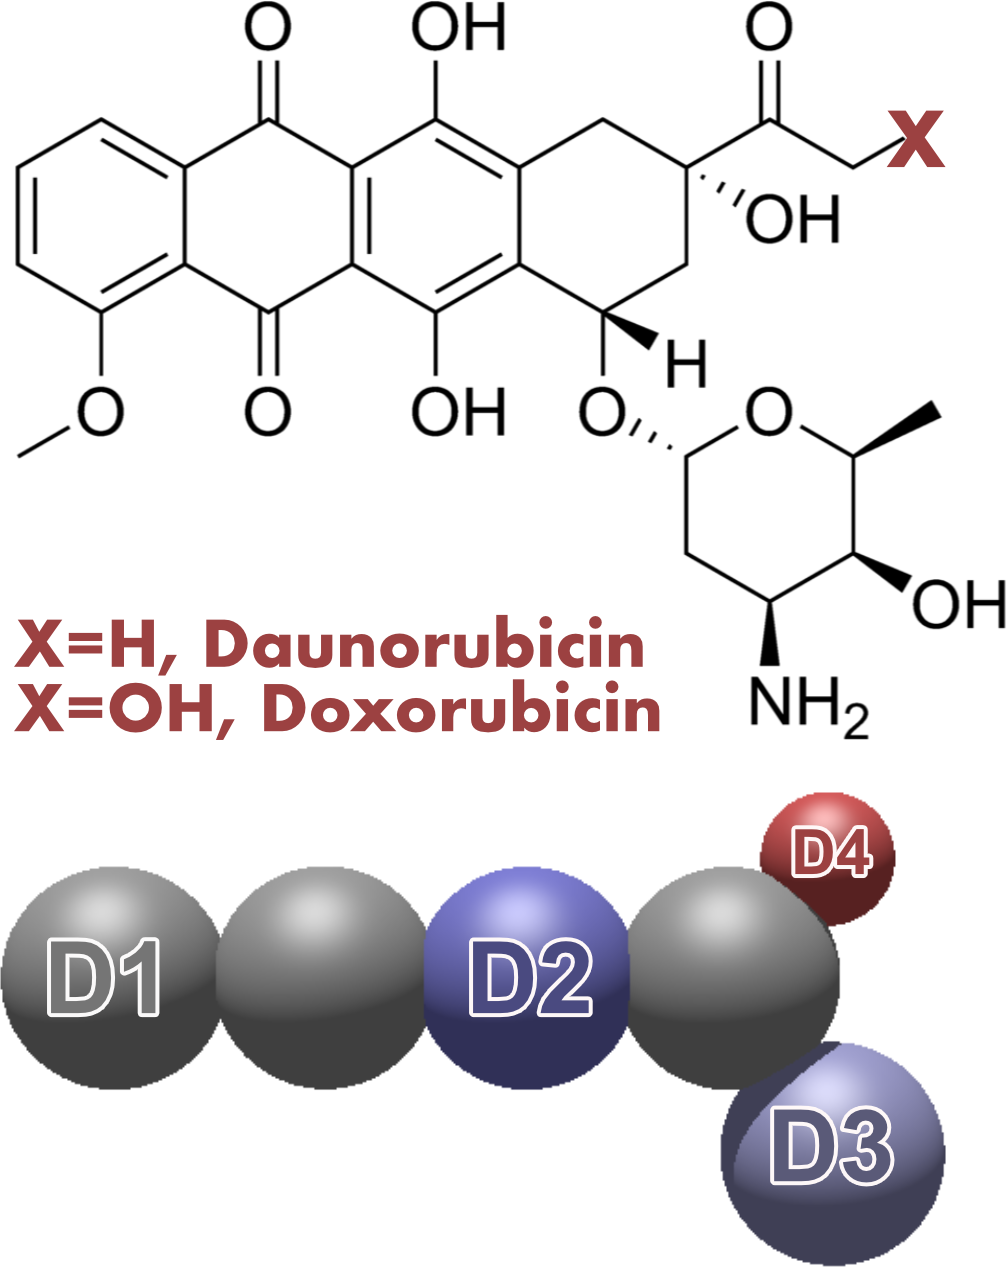
\includegraphics[width=0.35\linewidth]{Figures/graph-gel/dauno-doxo.png}
\caption{Estructura quí\'imica (arriba) y modelo de grano grueso (abajo) aplicado para describir daunorrubicina y doxorrubicina.
	Los segmentos de grano grueso $D1-D4$ se describen en la tabla \ref{table:gel:drugs}.}
\label{fig:gel:dauno-doxo}
\end{figure}


Consideraremos la absorci\'on de los f\'armacos quimioterap\'euticos Daunorrubicina (Dauno) y Doxorrubicina (Doxo) en nuestros microgeles P(NIPAm-MAA) en diferentes condiciones.
El modelo molecular aplicado para describir estos analitos se ilustra en la figura \ref{fig:gel:dauno-doxo} y la parametrizaci\'on se presenta en la tabla \ref{table:gel:drugs} \cite{PerezChavez2020}.

\begin{table}
%\small
%\begin{tabular}{lcS[table-format=-1]S[table-format=0.3]}
\centering
\begin{tabular}{|lccc|}
    \hline
    {CG unit} & {$pKa$} & {$q$ ($e$)} & {$v$ ($\text{nm}^3$)} \\
      \hline
$D1$ & - & 0 & 0.085\\
$D2$ & 7.34 & -1$^\ast$ & 0.085\\
$D3$ & 9.46 & +1$^\ast$ & 0.085\\ 
$D4$ (Doxo) & 8.46 & -1$^\ast$ & 0.035\\
$D4$ (Dauno) & - & 0 & 0.035 \\
    \hline
  \end{tabular}
 \caption{Porpediades moleculares para las distintas unidades de grano grueso usadas para el modelado de las drogas Daunorubicina y Doxorubicina. (ver figura \ref{fig:gel:dauno-doxo}).
\footnotesize ($^\ast$ Para unidades ionizables.)}
\label{table:gel:drugs} 
\end{table}




\section{Resultados y discusi\'on}
%%%%%%%%%%%%%%%%%%%%%%%%%%%%%%%%%%%%%%%%%%%%%%%%%%%%%%%%%%%%%%%%%%%%%



%%%%%%%%%%%%%%%%%%%%%%%%%%%%%%%%%%%%%%%%%%%%%%%%%%%%%%%%%%%%%%%%%%%%%
\subsection{Respuesta al pH y la concentraci\'on de sal}\label{sec:gel:pH_salt}
%%%%%%%%%%%%%%%%%%%%%%%%%%%%%%%%%%%%%%%%%%%%%%%%%%%%%%%%%%%%%%%%%%%%%


\begin{figure}[!ht]
\centering
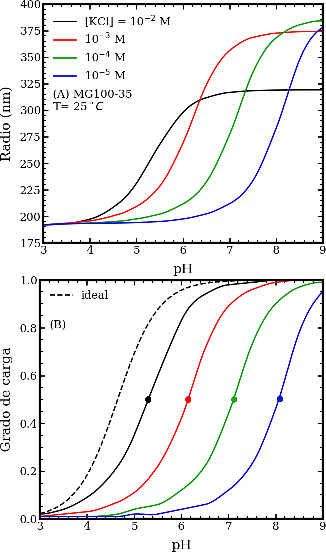
\includegraphics[width=0.5\linewidth]{Figures/graph-gel/R-pH.pdf}
\caption{Gr\'afico de tama\~no de microgel (A) y grado de carga (B) en funci\'on del pH para soluciones que tienen diferentes concentraciones de sal y $T=25 ^\circ C$.
	Las cadenas de pol\'imero en el microgel MG100-35 son $n_{ch}=100$-long. y tienen $35\% $ MAA.
	La curva de  punteada en el panel B es la disociaci\'on ideal del \'acido metacr\'ilico ($pKa=4.65$).
	Los c\'irculos de color en las curvas del panel A marcan el pKa aparente del microgel.}
\label{fig:gel:R-pH}
\end{figure}

En esta secci\'on, describiremos el comportamiento de los microgeles en respuesta a cambios en la composici\'on de la soluci\'on. Nos enfocaremos en temperaturas por debajo de la temperatura cr\'itica del PNIPAm, donde el gel experimenta un colapso. El efecto de la temperatura se evaluar\'a en la secci\'on \ref{sec:gel:temperature}.

La Figura \ref{fig:gel:R-pH}A muestra el tama\~no del microgel (radio, $R$) en funci\'on del pH para diferentes concentraciones de sal. Los microgeles de P(NIPAm-MAA) se hinchan al aumentar el pH. A medida que el pH se incrementa, un n\'umero creciente de unidades  de $MAA$ se desprotona y, por lo tanto, se cargan el\'ectricamente. La Figura \ref{fig:gel:R-pH}B muestra c\'omo la fracci\'on de $MAA$ cargados ($f$: grado de carga; ver ec. \ref{eq:gel:fcharge}) depende del pH de la soluci\'on. El hinchamiento observado en el panel A, que surge al aumentar el pH, es una respuesta a las crecientes repulsiones dentro del microgel, resultado del aumento de la carga el\'ectrica en la red polim\'erica, como se observa en el panel B.

El inicio de la transici\'on de este hinchamiento se desplaza a valores de pH m'as altos cuando se reduce la concentraci\'on de sal (ver Figura \ref{fig:gel:R-pH}A). Las curvas de disociaci\'on de protones del panel B presentan el mismo desplazamiento a pH m\'as altos, en comparaci\'on con el comportamiento ideal de un mon\'omero de $MAA$ aislado en soluci\'on diluida. Hemos discutido este comportamiento en el cap\'itulo \ref{Chapter-film}, en la secci\'on \ref{sec:film:respuesta-pH}.

El pKa aparente es el pH en el cual la mitad de los segmentos de $MAA$ se desprotonan, y este valor cuantifica el comportamiento de carga del microgel (ver Figura \ref{fig:gel:R-pH}B), as\'i como la transici\'on de expansi\'on (como se observa en el panel A, marcado con c\'irculos en $pH=pKa$). Los pKa aparentes de la Figura \ref{fig:gel:R-pH}B se muestran en la Tabla \ref{table:gel:pKa_app}.





\begin{table}[!htb]
\centering
\small
  \begin{tabular}{|cc|}
    \hline
      [KCl] (M)&  pKa apa. ($25 ^\circ C$)  \\
      \hline
    $10^{-5}$ & 8.10  \\
    $10^{-4}$ & 7.15 \\
    $10^{-3}$ & 6.15 \\
    $10^{-2}$ & 5.35 \\
    %\azul $10^{-1}$ & \azul 4.80 \\
    ideal (pKa) &  $4.65$  \\
    \hline
  \end{tabular}
 \caption{ pka's aparente de la fig. \ref{fig:gel:R-pH} para un gel MG100-35 a $25 ^\circ C$.}
\label{table:gel:pKa_app} 
\end{table}


Una concentraci\'on relativamente alta de iones de sal dentro del microgel da como resultado el apantallamiento de las repulsiones electrost\'aticas entre los segmentos $MAA$ cargados; estas interacciones repulsivas se vuelven de corto alcance.
Cuando el pH de la soluci\'on aumenta, la disociaci\'on de los segmentos de $MAA$ sucede sin un alto costo energ\'etico originado por las repulsiones electrost\'aticas.
En estas condiciones, la desprotonaci\'on de $MAA$, inducida por la energ\'ia qu\'imica libre (equilibrio \'acido-base), se aproxima al comportamiento ideal o de una soluci\'on diluida (compar\'andose los casos de alta concentraci\'on salina con la curva de l\'inea punteada en la Figura \ref{fig:gel:R-pH}B).

Por el contrario, a bajas concentraciones de sal, el efecto de apantallamiento se debilita y las repulsiones electrost\'aticas dentro de la red son de mayor alcance.
Incluso si hay pocas cargas y distantes en la red, interactuar\'an entre s\'i.
Para reducir la contribuci\'on energ\'etica de tales repulsiones electrost\'aticas hay una disminuci\'on significativa a que las unidades $MAA$ se carguen en condiciones de baja salinidad;
en consecuencia, el pKa aparente aumenta.
El precio a pagar es aumentar la energ\'ia qu\'imica libre, cuya contribuci\'on se minimiza cuando el grado de protonaci\'on es ideal.




\begin{figure*}[!htb]
	\centering
	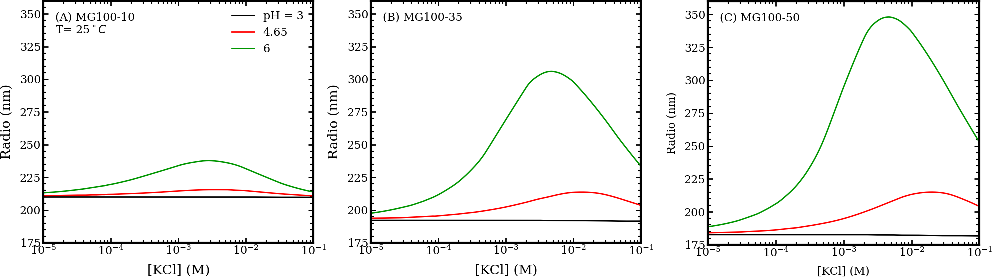
\includegraphics[width=1\linewidth]{Figures/graph-gel/R-cs.pdf}
	\caption{Gr\'afico del tama\~no del microgel en funci\'on de las concentraciones de sal para diferentes soluciones de pH y $T=25 ^\circ C$.
		Los paneles corresponden a microgeles MG-100 (longitud de cadena, $n_{ch}=100$) que tienen fracciones MAA: $10\%$ (A), $35\%$ (B) y $50\%$ (C).}
	\label{fig:gel:R-cs}
\end{figure*}


La Figura \ref{fig:gel:R-cs} ilustra c\'omo el tama\~no de los microgeles de P(NIPAm-MAA) depende de la concentraci\'on de sal para diferentes valores de pH.
A una salinidad relativamente alta, estos microgeles se hinchan con el aumento de la concentraci\'on de sal, lo que es consistente con los resultados de dispersi\'on de luz din\'amica (DLS) reportados por \citet{Wong2009} para microgeles P(NIPAm-MAA) y concentraciones de KCl en el rango de $0.1-0.5\,M$.

Las curvas de la Figura \ref{fig:gel:R-cs} muestran un comportamiento reentrante, en el que el tama\~no primero aumenta y luego disminuye al aumentar la concentraci\'on de sal.
Esta respuesta no monot\'onica es m\'as acentuada cuando la carga del pol\'imero aumenta debido a un mayor contenido de unidades de $MAA$ (observado en los diferentes paneles de la Figura \ref{fig:gel:R-cs}).

Se han informado transiciones de hinchamiento-deshinchamiento con concentraciones de sal variables en una variedad de sistemas polim\'ericos reguladores de carga.
El grosor de las capas de poli\'acidos d\'ebiles anclados es una funci\'on no monot\'onica de la concentraci\'on de sal de la soluci\'on seg\'un lo predicho por la teor\'ia del campo medio autoconsistente \cite{Israels1994, Lyatskaya1995, Zhulina1995, Gong2007}, lo cual ha sido confirmado por resultados experimentales \cite{Wu2007}.
De manera similar, los resultados te\'oricos predicen que el tama\~no de los polielectrolitos d\'ebiles ramificados en forma de estrella muestra un m\'aximo en funci\'on de la concentraci\'on de sal en la soluci\'on \cite{Borisov1998, KleinWolterink2002}.
Tambi\'en se ha predicho que el espesor de las pel\'iculas de poli\'acidos d\'ebiles entrecruzados mostrar\'a este comportamiento de hinchamiento reentrante \cite{Longo2014JCP}.






En este mismo sentido, se ha predicho una transici\'n de deshinchaci\'on a hinflaci\'on impulsada por la concentraci\'on de sal para los nanogeles de polielectrolitos fuertes \cite{jha2012understanding}. Este comportamiento, en el caso de los polielectrolitos ``quencheados", se atribuye a los efectos de volumen excluidos de los iones absorbidos a altas concentraciones salinas.

M\'as relevante para nuestro estudio, son los resultados te\'oricos de una transici\'on reentrante de hinchaci\'on a colapso para microgeles sensibles al pH y al calor \cite{polotsky2013collapse}. \citet{polotsky2013collapse} explica que el aumento de la concentraci\'on de sal promueve inicialmente la disociaci\'on de carga de los grupos \'acidos d\'ebiles hasta alcanzar la saturaci\'on, momento en el cual el grado de disociaci\'on alcanza el valor ideal. M\'as all\'a de este punto, el aumento de la concentraci\'on de sal en la soluci\'on solo mejora el apantallamiento de las repulsiones electrost\'aticas y, por lo tanto, el microgel se deshincha.

Experimentalmente, \citet{CaprilesGonzalez2008} informaron sobre el hinchamiento no monot\'onico de los microgeles de poli(NIPAm-\emph{co}-AA) (P(NIPAm-AA)) en funci\'on de la concentraci\'on de NaCl utilizando t\'ecnicas de DLS.




\begin{figure}[!tb]
	\centering
	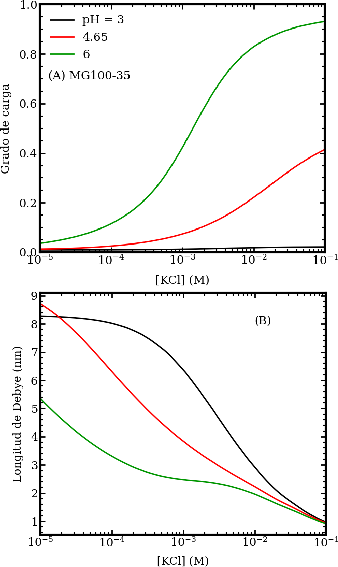
\includegraphics[width=0.5\linewidth]{Figures/graph-gel/f-cs.pdf}
	\caption{Curvas del grado de carga MAA (A) y la longitud de Debye (B) dentro de los microgeles MG100-35 en funci\'on de la concentraci\'on de sal para diferentes valores de pH.
		Estos resultados corresponden a las condiciones de figura \ref{fig:gel:R-cs}B.}
	\label{fig:gel:f-cs}
\end{figure}

El aumento de la concentraci\'on de sal de la soluci\'on tiene dos efectos opuestos sobre las propiedades del microgel. Por un lado, aumenta el apantallamiento de interacciones de carga a medida que se cargan los iones dentro del gel; las repulsiones electrost\'aticas entre los mon\'omeros de $MAA$ cargados est\'an cada vez m\'as protegidas. El alcance efectivo de estas repulsiones se acorta, favoreciendo el deshinchamiento. Por otro lado, este apantallamiento permite una mayor desprotonaci\'on de los mon\'omeros de $MAA$, promovida por el equilibrio \'acido-base. La disociaci\'on de carga favorece el hinchamiento para reducir las repulsiones electrost\'aticas.

La figura \ref{fig:gel:f-cs} ilustra este doble efecto de aumentar la concentraci\'on de sal en la soluci\'on, lo que conduce al comportamiento de hinchamiento-deshinchamiento. El panel A muestra que la carga del microgel aumenta mon\'otonamente con la concentraci\'on de sal. En el panel B, usamos la longitud de Debye para cuantificar la extensi\'on de las interacciones electrost\'aticas.% (consulte la ecuaci'on \ref{eq:debye_length} en el suplemento). 
El alcance efectivo de estas interacciones se acorta dentro del microgel a medida que aumenta la concentraci\'on de sal. Se puede observar en la figura \ref{fig:gel:f-cs} que en condiciones de pH 3 la carga dentro del microgel es insignificante, lo que resulta en un hinchamiento muy poco apreciable en la figura \ref{fig:gel:R-cs}B.

Esta teor\'ia requiere que el interior del microgel sea de carga neutra. La congujaci\'on de cargas y contraiones debe estar equilibrada. \citet{Claudio2009} demostr\'o que esta es una aproximaci\'on razonable cuando el microgel es m\'as grande que $R = 125,\text{nm}$ y tiene un 50\% de mon\'omeros cargados. Los microgeles P(NIPAm-MAA) aqu\'i planteados son m\'as grandes que ese tama\~no en la mayor\'ia de las condiciones, particularmente cuando el pH est\'a por encima del pKa aparente y la mayor\'ia de los grupos $MAA$ est\'an desprotonados. Adem\'as, los iones de sal se absorben dentro del microgel para reforzar dicha restricci\'on, lo que permite que los segmentos de $MAA$ se desprotonen y se carguen el\'ectricamente. Describimos este efecto como el apantallamiento de las repulsiones electrost\'aticas entre los grupos de $MAA$, que es un concepto que hemos discutido con anterioridad.


\subsection{Respuesta a la Temperatura}\label{sec:gel:temperature}
%%%%%%%%%%%%%%%%%%%%%%%%%%%%%%%%%%%%%%%%%%%%%%%%%%%%%%%%%%%%%%%%%%%%%

\begin{figure*}[!htb]
	\centering
	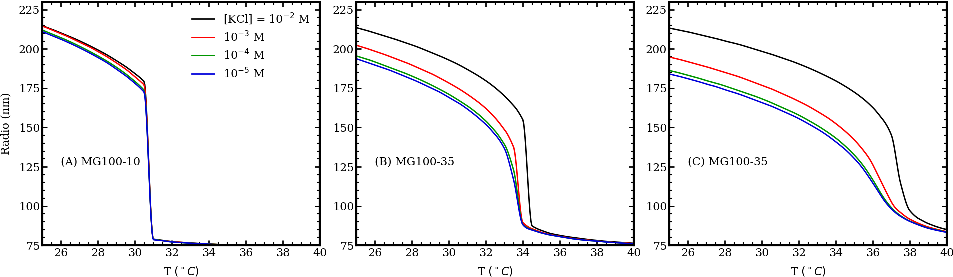
\includegraphics[width=1\linewidth]{Figures/graph-gel/R-T.pdf}
	\caption{Gr\'afico del tama\~no del microgel en funci\'on de la temperatura para diferentes concentraciones de sal en soluci\'on y $pH~4,65$.
		Los paneles corresponden a microgeles MG-100 (longitud de cadena, $n_{ch}=100$) que tienen diferentes fracciones de $MAA$: $10\%$ (A), $35\%$ (B) y $50\%$ (C).}
	\label{fig:gel:R-T}
\end{figure*}

Discutido el efecto del pH y la concentraci\'on de sal, ahora nos enfocaremos en mostrar la respuesta de los microgeles de P(NIPAm-MAA) frente a cambios en la temperatura.
En cada panel de la figura \ref{fig:gel:R-T} se muestra el tama\~no de tres geles MG-100 como funci\'on de la temperatura a distintas concentraciones salinas.
A baja temperatura, estos microgeles muestran un estado relativamente hinchado, mientras que a altas temperaturas se produce un estado colapsado (alta densidad de pol\'imero).

Esto \'ultimo ocurre dado que el NIPAm adquiere un comportamiento hidrof\'obico por encima de su temperatura de transici\'on cr\'itica inferior (LCST por sus siglas en ingl\'es), expulsando el solvente de su interior y colapsando su estructura \cite{sbeih2019structural}.
El tama\~no del gel en este estado es robustamente independiente de la concentraci\'on salina o el pH y posee un radio muy cercano al del microgel seco (ver tabla \ref{table:gel:optimal-R}).

Por otro lado, el estado hinchado del gel est\'a dominado por las repulsiones electrost\'aticas entre los segmentos de $MAA$ cargados y los contraiones absorbidos, como fue descrito en la secci\'on \ref{sec:gel:pH_salt}.
El tama\~no y la carga del microgel son funciones mon\'otonamente decrecientes de la temperatura.


\begin{figure}[!htb]
	\centering
	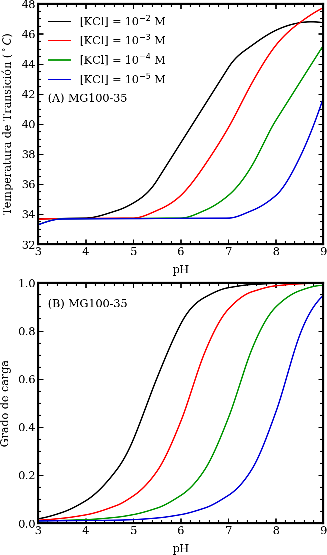
\includegraphics[width=0.5\linewidth]{Figures/graph-gel/Tpt-pH.pdf}
	\caption{Gr\'aficos que muestran la temperatura de transici\'on de volumen $T_{TV}$ (A) y la fracci\'on de $MAA$ cargado a esta temperatura (B) en funci\'on del pH para diferentes concentraciones de sal.
		Este microgel P(NIPAm-MAA) tiene una longitud de cadena de $n_{ch}=100$ y un MAA de $35\%$.}
	\label{fig:gel:Tpt-pH}
\end{figure}


En la mayor\'ia de las condiciones, pero no en todas, la transici\'on entre estos dos estados del microgel es brusca y ocurre en un rango estrecho alrededor de una temperatura bien definida, que definimos como Temperatura de Transici\'on de Volumen ($T_{TV}$). Comparando los diferentes paneles de la figura \ref{fig:gel:R-T}, vemos que aumentar el contenido de $MAA$ de los microgeles conduce a una transici\'on m\'as suave alrededor de $T_{TV}$.

La figura \ref{fig:gel:Tpt-pH}A muestra que la $T_{TV}$ aumenta con el pH y la concentraci\'on de sal. Estos resultados son consistentes con los experimentos de DLS que muestran que la temperatura de transici\'on volum\'etrica de los microgeles P(NIPAm-MAA) aumenta con el pH \cite{Kleinen2008}, lo que tambi\'en se ha observado para los microgeles P(NIPAm-AA) \cite{CaprilesGonzalez2008}. Se ha definido $T_{TV}$ como el punto de inflexi\'on de las curvas $R(T)$ de la figura \ref{fig:gel:R-T} entre los estados hinchado y colapsado \cite{Kratz2001}.

El panel B de la figura \ref{fig:gel:Tpt-pH} muestra el grado de carga de los segmentos de $MAA$ en el $T_{TV}$. Existe una clara correlaci\'on entre la dependencia de $T_{TV}$ con el pH y la salinidad, y el estado de carga del microgel en las condiciones VPT. La temperatura de transici\'on aumenta con el pH y la concentraci\'on de sal, al igual que la carga de la red de pol\'imeros.

A diferencia de este comportamiento, el VPTT de los microgeles basados en PNIPAm permanentemente cargados disminuye con la concentraci\'on de sal \cite{Lopez2020}. En este caso, la carga del pol\'imero permanece constante, mientras que la incorporaci\'on de iones de sal solo debilita las repulsiones electrost\'aticas entre las cargas.

\begin{figure}[!tb]
	\centering
	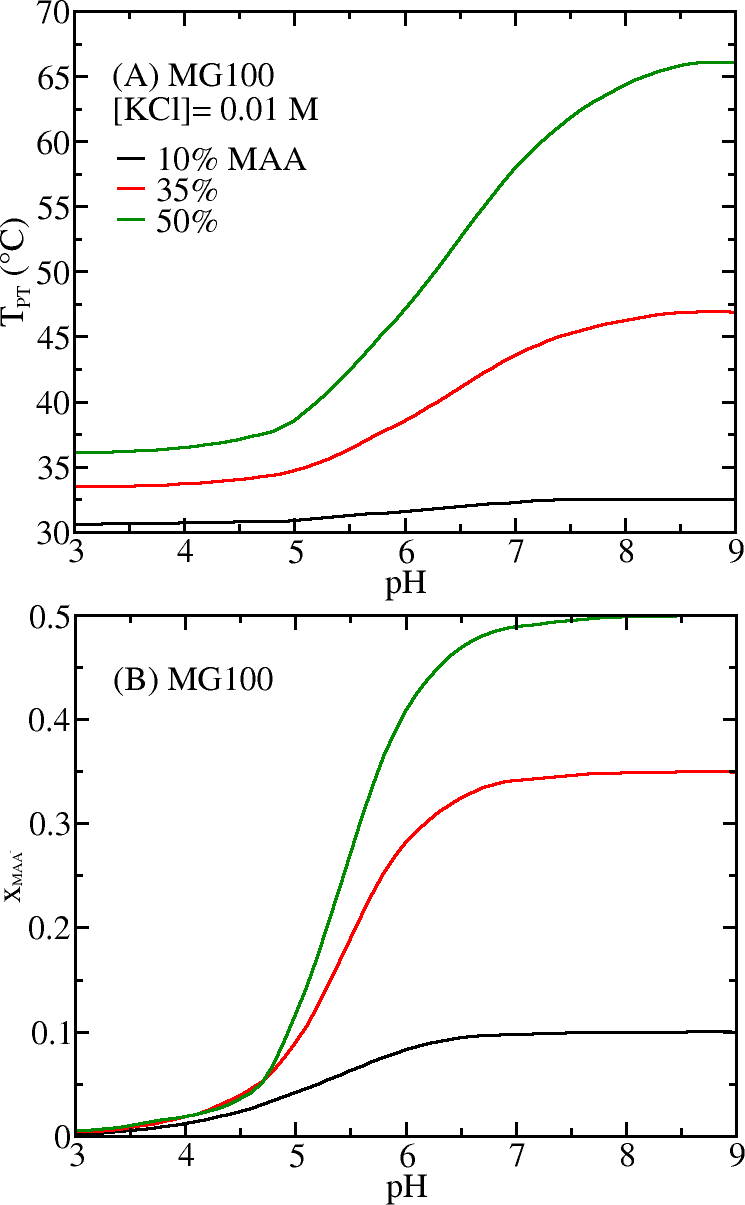
\includegraphics[width=0.5\linewidth]{Figures/graph-gel/Tpt-pH_MAA.png}
	\caption{(A) Gr\'afico de temperatura de transici\'on $T_{TV}$ en funci\'on del pH para microgeles MG-100 (longitud de cadena de pol\'imero, $n_{ch}=100$ segmentos) que tienen diferentes contenidos de MAA; $[KCl]=0.01 M$;
	(B) Fracci\'on de segmentos cargados $x_{MAA^-}=\frac{N_{MAA^-}}{N_{seg}}$ en funci\'on del pH para las mismas condiciones del panel A (\emph{i.e.} , en el $T_{TV}$); $x_{MAA^-}$ es proporcional a la carga total del pol\'imero; $N_{seg}$ es el mismo para todos los microgeles.}
	\label{fig:gel:Tpt_MAA}
\end{figure}

Los resultados de la figura \ref{fig:gel:Tpt-pH} muestran que la temperatura de transici\'on est\'a controlada por la cantidad de carga dentro del microgel. De hecho, aumentar el contenido de MAA tiene el mismo efecto de desplazar el VPTT a valores m\'as altos, como se observa en la figura \ref{fig:gel:Tpt_MAA}A. Una vez m\'as, este comportamiento resulta de una estructura polim\'erica m\'as cargada.

Para comparar el estado de carga de microgeles con diferentes contenidos de $MAA$, utilizamos la fracci\'on total de mon\'omeros cargados:

\begin{equation}
	x_{MAA^-}=\frac{N_{MAA^-}}{N_{seg}}=f x_{MAA}
\end{equation}

Donde $N_{MAA^-}$ es el n\'umero de segmentos MAA desprotonados, todas las dem\'as cantidades se han definido en la secci\'on \ref{sec:gel:theory}. $x_{MAA^-}$ es proporcional a la carga total de la red de microgel, y debido a que todos los microgeles tienen el mismo n\'umero total de segmentos, la constante proporcional es la misma para todos los contenidos de $MAA$ considerados. La figura \ref{fig:gel:Tpt_MAA}B muestra que existe una clara correlación entre $T_{TV}$ y la carga total del microgel (dada por $x_{MAA^-}$) al cambiar el pH o el contenido de $MAA$ del pol\'imero.


%%%%%%%%%%%%%%%%%%%%%%%%%%%%%%%%%%%%%%%%%%%%%%%%%%%%%%%%%%%%%%%%%%%%%
\subsection{Efecto del grado de entrecruzamiento} \label{sec:gel:entrecruzamiento}
%%%%%%%%%%%%%%%%%%%%%%%%%%%%%%%%%%%%%%%%%%%%%%%%%%%%%%%%%%%%%%%%%%%%%


\begin{figure*}[!tb]
	\centering
	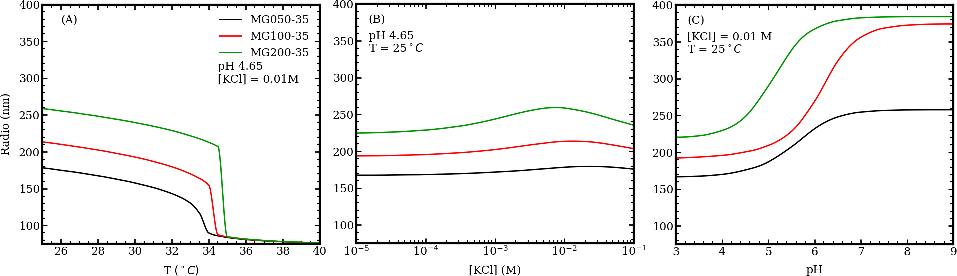
\includegraphics[width=1\linewidth]{Figures/graph-gel/R-all_xlink.pdf}
	\caption{Gr\'afico del tama\~no del microgel en funci\'on de la temperatura, la concentraci\'on de sal y el pH (paneles A, B y C respectivamente).
		Diferentes curvas corresponden a microgeles con segmentos de $50$ (MG050), $100$ (MG100) y $200$ (MG200) por cadena de pol\'imero, todos con $35\%$ MAA.}
	\label{fig:gel:R_xlink}
\end{figure*}

En esta instancia vamos a analizar c\'omo el grado de entrecruzamiento de la red polim\'erica afecta el comportamiento previamente descrito de nuestro gel. Consideramos microgeles con segmentos de $50$, $100$ y $200$ por cadena, manteniendo el mismo n\'umero total de segmentos. A medida que la cantidad de segmentos por cadena disminuye, aumenta el grado de entrecruzamiento en el microgel. La figura \ref{fig:gel:R_xlink} muestra la respuesta de los microgeles con un porcentaje de $MAA$ del $35\%$ ante cambios de temperatura (panel A), concentraci\'on de sal (panel B) y pH (panel C).

Los microgeles con menor grado de entrecruzamiento (mayor n\'umero de segmentos por cadena) presentan un mayor grado de hinchamiento. Este comportamiento de los microgeles P(NIPAm-MAA) ha sido confirmado experimentalmente \cite{khan2013preparation}. Cualitativamente, la respuesta a la concentraci\'on de sal y al pH es similar para todas las longitudes de cadena consideradas (paneles B y C de la figura \ref{fig:gel:R_xlink}, respectivamente). Una observaci\'on interesante es que la disminuci\'on del grado de entrecruzamiento conduce a una transici\'on de volumen m\'as brusca a medida que aumenta la temperatura (figura \ref{fig:gel:R_xlink}A), y adem\'as, la temperatura de transici\'on de volumen ($T_{TV}$) aumenta. Estos resultados son consistentes con los trabajos de \citet{li1989study} y \citet{wu1997volume}, quienes informaron un cambio en la transici\'on de volumen de NIPAm de continua a discontinua a medida que disminuye la concentraci\'on del entrecruzante en la s\'intesis.

En la figura \ref{fig:gel:R_xlink}, tambi\'en se observa que el aumento de la longitud de la cadena (disminuci\'on del grado de entrecruzamiento) desplaza la temperatura de transici\'on de volumen ($T_{TV}$) hacia valores m\'as altos. Esto concuerda con los resultados de la espectroscopía UV realizada por \citet{Lee2008} para los microgeles P(NIPAm-AA). Este comportamiento se observa en todo el rango de condiciones exploradas en este cap\'itulo.

La constante de fuerza de la contribuci\'on el\'astica a la energ\'ia libre es inversamente proporcional a la longitud de la cadena $n_{ch}$ (ver ecuaci\'on \ref{eq:gel:free-energy}). Al reducir el grado de entrecruzamiento, el microgel se hincha y se vuelve m\'as flexible, lo que permite una mayor carga en la red de pol\'imero. En consecuencia, se requiere una temperatura m\'as alta para inducir el colapso de la red de pol\'imero. Hemos demostrado que la temperatura de transici\'on de volumen ($T_{TV}$) est\'a fuertemente correlacionada con el grado de carga.

La presencia de unidades \'acidas acent\'uaa la dependencia de la $T_{TV}$ con la longitud de la cadena, ya que incorpora el equilibrio de protonaci\'on al balance energ\'etico. Sin embargo, este comportamiento es intr\'inseco a la interacci\'on entre las propiedades hidrof\'obicas y la elasticidad de la red polim\'erica. De hecho, la temperatura de transici\'on de los microgeles de PNIPAm puros tambi\'en aumenta con la longitud de la cadena, aunque el efecto es significativamente m\'as d\'ebil en ausencia de segmentos de $MAA$.



%%%%%%%%%%%%%%%%%%%%%%%%%%%%%%%%%%%%%%%%%%%%%%%%%%%%%%%%%%%%%%%%%%%%%
\subsection{Adsorci\'on de drogas}\label{sec:gel:ads-drogas}
%%%%%%%%%%%%%%%%%%%%%%%%%%%%%%%%%%%%%%%%%%%%%%%%%%%%%%%%%%%%%%%%%%%%%


Los microgeles polim\'ericos se han destacado como transportadores inteligentes de medicamentos debido a sus propiedades \'unicas. Estos sistemas nanoestructurados (en este caso microestrucutrados) ofrecen una plataforma vers\'atil para la encapsulaci\'on, protecci\'on y liberaci\'on controlada de sustancias bioactivas. Los microgeles pueden responder a est\'imulos externos,como hemos mostrados en las secciones anteriores,  como cambios de pH, temperatura y concentraci\'on de iones, lo que les permite liberar su carga terap\'eutica de manera selectiva y espec\'ifica en el sitio deseado. 

Por ejemplo, se sabe que el pH extracelular del tejido tumoral es m\'as bajo que el del tejido sano \cite{Gerweck1996}, lo que hace que los microgeles respondan al pH sean idoneos para la administraci\'on local de medicamentos contra el c\'ancer \cite{Dadsetan2013}.

Peppas \emph{et al.} han estudiado ampliamente los microgeles sensibles al pH basados en $MAA$ como transportadores inteligentes que pueden operar utilizando los diferentes niveles de acidez a lo largo del tracto digestivo y prevenir la degradaci\'on de f\'armacos en el est\'omago \cite{TorresLugo2002, Carr2010, DuranLobato2014, Sharpe2018}.

En esta secci\'on, evaluamos la capacidad de los microgeles P(NIPAm-MAA) para incorporar dos f\'armacos quimioterap\'euticos. En particular, investigamos las mejores condiciones para la encapsulaci\'on de f\'armacos en condiciones de laboratorio. Consideramos que la doxorrubicina (Doxo) y la daunorrubicina (Dauno) son dos de las antraciclinas importantes y ampliamente utilizadas en la quimioterapia para tratar una amplia gama de c\'anceres \cite{Panis2012, Carvalho2009, aubel1984daunorubicin,come1999dual}. Estas drogas se pueden seguir utilizando fluorescencia y adsorbancia, lo que las hace atractivas desde el punto de vista de la investigaci\'on \cite{Serpe2005, ThanHtun2009, PerezChavez2020}. Adem\'as, estos f\'armacos pueden adquirir carga positiva en la mayor\'ia de las condiciones, lo que puede facilitar su encapsulaci\'on en microgeles de pol\'imeros ani\'onicos \cite{Li2019}. \citet{Serpe2005} han estudiado la captaci\'on y liberaci\'on termicamente activadas de Doxo a partir de pel\'iculas capa por capa de microgeles de P(NIPAm-AA) y poli(clorhidrato de alilamina). M\'as recientemente, utilizando resonancia magn\'etica nuclear de lapso de tiempo, \citet{MartinezMoro2020} han descrito la interacci\'on entre Doxo y microgeles P(NIPAm-MAA) en diferentes condiciones.
\begin{figure}[!tb]
	\centering
	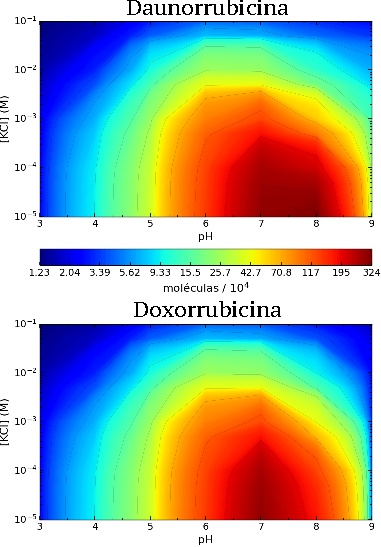
\includegraphics[width=0.55\linewidth]{Figures/graph-gel/drug_ads.pdf}
	\caption{Mapas en color que muestran el n\'umero de mol\'eculas de daunorrubicina (A) y doxorrubicina (B) absorbidas por microgel en funci\'on del pH de la soluci\'on y la concentraci\'on de sal.
		La concentraci\'on de f\'armaco en soluci\'on es $1mM$ y $T=25 ^\circ C$.
		el microgel P(NIPAm-MAA) tiene $n_{ch}=100$ de longitud de cadena y $35\%$ MAA (MG100-35).}
	\label{fig:gel:drug_ads}
\end{figure}


La figura \ref{fig:gel:drug_ads} ilustra el n\'umero de mol\'eculas de Dauno (panel A) y Doxo (panel B) dentro del microgel en relaci\'on con la concentraci\'on de sal y el pH de la soluci\'on. Se observa que las condiciones \'optimas para la encapsulaci\'on de estos f\'armacos terap\'euticos corresponden a una baja concentraci\'on de sal y un pH de 6 a 8. La reducci\'on en la concentraci\'on de sal favorece la absorci\'on. Tanto Dauno como Doxo presentan una carga neta de $+1$ a pH \'acido y neutro (ver la figura \ref{fig:gel:carga-drug_ads}).

\begin{figure}[!tb]
	\centering
	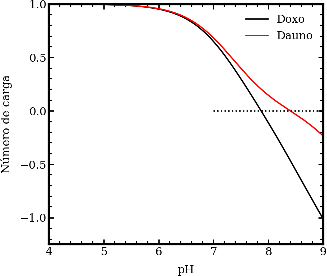
\includegraphics[width=0.9\linewidth]{Figures/graph-gel/drugs-Q.pdf}
	\caption{N\'umero de carga de las drogas estudiadas: Doxo y Dauno. La intersecci\'on con la l\'inea a puntos muestra el punto isolectrico de las mismas. Pasado este punto se da una inversi\'on en la carga de las drogas lo que conlleva a una respulsi\'on electrost\'atica con los segmentos cargados de $MAA$ del microgel. }
	\label{fig:gel:carga-drug_ads}
\end{figure}

Como resultado, la absorci\'on de Dauno y Doxo tiene que competir con la absorci\'on de iones de potasio para neutralizar la carga negativa de la red del pol\'imero (\citet{PerezChavez2020}). En la figura \ref{fig:gel:f-cs}, se observa que en ausencia de un f\'armaco disuelto, la carga del microgel disminuye a medida que se reduce la concentraci\'on de sal, lo que aparentemente entra en conflicto con la mejora de la absorci\'on observada en la figura \ref{fig:gel:drug_ads} bajo estas condiciones. Sin embargo, despu\'es de la absorci\'on del f\'armaco, el grado de carga de los segmentos de MAA aumenta significativamente, especialmente en condiciones de baja concentraci\'on de sal. Adem\'as, es importante destacar que este comportamiento est\'a particularmente asociado con la relativamente alta concentraci\'on de f\'armaco considerada en estos resultados ($1\, mM$).

La fracci\'on de segmentos de $MAA$ cargados negativamente en el pol\'imero aumenta con el pH, lo que explica por qu\'e tambi\'en aumenta la absorci\'on de Dauno/Doxo en condiciones \'acidas. Sin embargo, en condiciones alcalinas, la carga neta positiva de estos f\'armacos disminuye con el aumento del pH, lo que desfavorece su absorci\'on. Por lo tanto, la absorci\'on de Dauno/Doxo es una funci\'on no mon\'otona del pH.

En nuestro modelo, los puntos isoel\'ectricos de Dauno y Doxo son 8.4 y 7.9, respectivamente ver fig. \ref{fig:gel:carga-drug_ads}. La figura \ref{fig:gel:drug_ads} muestra que la adsorci\'on de ambas mol\'eculas puede ser significativa alrededor y por encima de estos valores de pH. En otras palabras, hay una adsorci\'on considerable de mol\'eculas con carga negativa dentro de la red de nuestro gel con carga similar. Aunque estas mol\'eculas est\'an cargadas negativamente en la fase de soluci\'on, la absorci\'on ocurre porque el pH disminuye dentro del microgel, lo que permite que los f\'armacos regulen su carga el\'ectrica y permanezcan cargados positivamente dentro del microgel (fig. \ref{fig:gel:drug_pH}).


\begin{figure}[!tb]
	\centering
	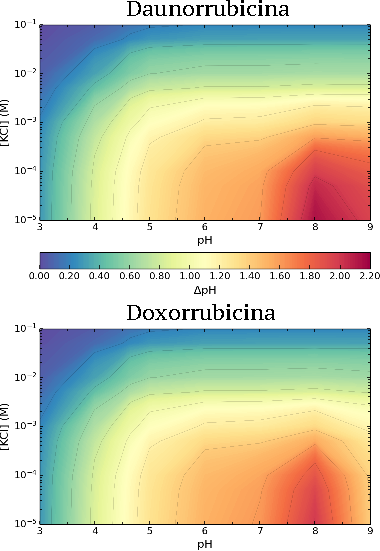
\includegraphics[width=0.55\linewidth]{Figures/graph-gel/drug_pH.pdf}
	\caption{Mapas en color que muestran el cambio en el pH dentro del microgel, $\Delta pH = pH - pH_{GEL}$ en funci\'on de sal y el pH de la soluci\'on para daunorrubicina (A) y doxorrubicina (B). Estos cambios son reportados para las mismas condiciones de \ref{fig:gel:drug_ads}, es decir:
		La concentraci\'on de f\'armaco en soluci\'on es $1mM$ y $T=25 ^\circ C$.
		el microgel P(NIPAm-MAA) tiene $n_{ch}=100$ de longitud de cadena y $35\%$ MAA (MG100-35).}
	\label{fig:gel:drug_pH}
\end{figure}

El punto isoel\'ectrico m\'as bajo de la doxorrubicina se debe a la desprotonaci\'on de su grupo hidroxilo sustituyente (v\'ease  el segmento $D4$ en la figura \ref{fig:gel:dauno-doxo} y tabla \ref{table:gel:drugs}). Como resultado de esta carga negativa adicional en condiciones alcalinas, el rango de pH de adsorci\'on es ligeramente m\'as amplio para la daunorrubicina.

\section{Conclusiones}

En este cap\'itulo mostramos una teor\'ia termodin\'amica  para un sistema compuesto de dos fases con el cual se describe la respuesta de diferentes nano/microgeles de P(NIPAm-MAA) a los cambios en el pH, la concentraci\'on de sal y la temperatura.
Estas part\'iculas suaves se hinchan con el aumento del pH, lo cual es resultado de las repulsiones electrost\'aticas entre los segmentos cargados de MAA a medida que se disocian.
Este comportamiento de hinchamiento est\'a controlado por la carga \cite{FernandezNieves2000}.
El inicio de esta transici\'on impulsada por el pH se puede caracterizar adecuadamente utilizando el pKa aparente de los segmentos de MAA, que se desplaza a valores de pH m\'as altos a medida que disminuye la concentraci\'on de sal en la soluci\'on.

A pH constante y por debajo de la temperatura de transici\'on de fase inferior cr\'itica (LCST) del PNIPAm, el tama\~no de estos microgeles es una funci\'on no mon\'otona de la concentraci\'on de sal.
El aumento de la salinidad de la soluci\'on puede provocar tanto hinchamiento como deshinchamiento, dependiendo del rango de concentraci\'on de sal.
Esta transici\'on de hinchamiento-deshinchamiento inversa surge como resultado de la competencia entre los efectos opuestos del aumento de la concentraci\'on de sal en los sistemas de polielectrolito d\'ebil, que tanto promueve la disociaci\'on de la carga como mejora el apantallamiento de las repulsiones electrost\'aticas.


A medida que aumenta la temperatura, se produce una transici\'on de fase de volumen diferente que est\'a asociada a la hidrofobicidad intr\'inseca del PNIPAm por encima de su LCST.
La temperatura de transici\'on de fase de volumen de estos microgeles depende de la cantidad de MAA en el pol\'imero, el grado de entrecruzamiento, el pH de la soluci\'on y la concentraci\'on de sal.
Cambiar estas variables independientes y/o los par\'ametros de dise\~no son formas de modificar el estado de carga del microgel.
El mensaje principal de este cap\'itulo es que la cantidad de carga en la estructura del pol\'imero controla la temperatura de transici\'on de fase de volumen de los microgeles multiresponsivos.

Tambi\'en hemos evaluado la capacidad de estes microgeles para encapsular dos f\'armacos quimioterap\'euticos t\'ipicos con carga positiva.
El mejor enfoque para mejorar la partici\'on de estos f\'armacos en el microgel es reducir la concentraci\'on de sal en la soluci\'on.
M\'as sorprendente es el hecho de que las mejores condiciones de encapsulaci\'on corresponden a valores de pH alrededor o por encima de los puntos isoel\'ectricos de estos f\'armacos, donde estas mol'eculas tienen carga negativa en la soluci\'on de encapsulaci\'on. 